%! Author = ruochongli
%! Date = 2023/3/12

% Preamble
\documentclass[./main.tex]{subfiles}

% Packages

% Document
\begin{document}
    \section{Application}
    \subsection{Factors of the Model}

    In our model, there are many factors which needs to be defined when the model is being used to work out real problem.

    Firstly, we need to decide the usage of the land.
    In the given condition, the land can be used to build outdoor sports complexes, cross-country skiing facilities,
    crop farms, grazing farms/ranches, regenerative farms, solar arrays, agrivoltaic farms and agritourist centers.
    If the model is used in different condition, other usage such as factories, urban lands, greenbelts, etc.
    can also be involved.

    Then, there are the natural and human influence to be deliberate.
    What presented in the basic information of problem is geographic factors including elevation, slope, aspect, tree and land cover data.

    Additionally, we found the information of rainfall, temperature, soil quality, illumination time, visitors flow rate, population growth, etc.
    on the government websites and other authorized sources.
    More factors can be chosen or canceled when encountering different condition with different requirements.
    The proportion of the natural factors and human factors can also be modified to accord with the need.

    \subsection{Factor Quantification and Function Design}

    After considering the factors qualitatively, we need to quantify these factors and connect them to our ultimate goal.
    In this problem, the ultimate goal is to gain large profit through time, so we need to figure out the conversion
    relationship between factors mentioned above, time and profit.
    For example, the pollution factor could gain negative impact to the facility because the damage to environment
    could decrease the total production of agriculture, push away the tourists and affect the sustainability of the
    development of the entire property.
    The academic literature indicates that the damage to the environment and the concentration of pollution are in
    direct ratio, while the concentration at any position outside the pollution source can be calculated according to the time fractional diffusion equation.
    Thus, the weakening effect of pollution can be quantified.

    When considering other factors like visitors flow rate, which could bring positive effect to the tourism, the corresponding function would change and likely to be a positive ratio function.

    Further expansion can be similarly produced according to other specific needs.

    \subsection{The Verification of Application to the Given Problem}

    To verify the model, we first decide three part in Red Creek to build two kinds of facilities, and decide the solution according to our common sense.
    Then, we put the data we found into our algorithm and respectively calculate the absolute profit coefficient $P$.
    In contrast to the reasonable solution, we swap the position of the two facilities, which would be very unreasonable, and the output of the algorithm should be considerably lower than the previous result.
    By comparing this, we could roughly make out the reliability of the algorithm.

    The first pair of facility is the cross-country skiing facility and the crop farm.
    We divide three parts of the land according to its slope.
    We first put the cross-country skiing facility to the single one with greater slope, while the crop farms were
    put to gentler lands.
    Then we swap them.
    The detailed configurations are as follows:

    \begin{figure}[H]
        \centering
        \begin{minipage}{0.3\linewidth}
            \centering
            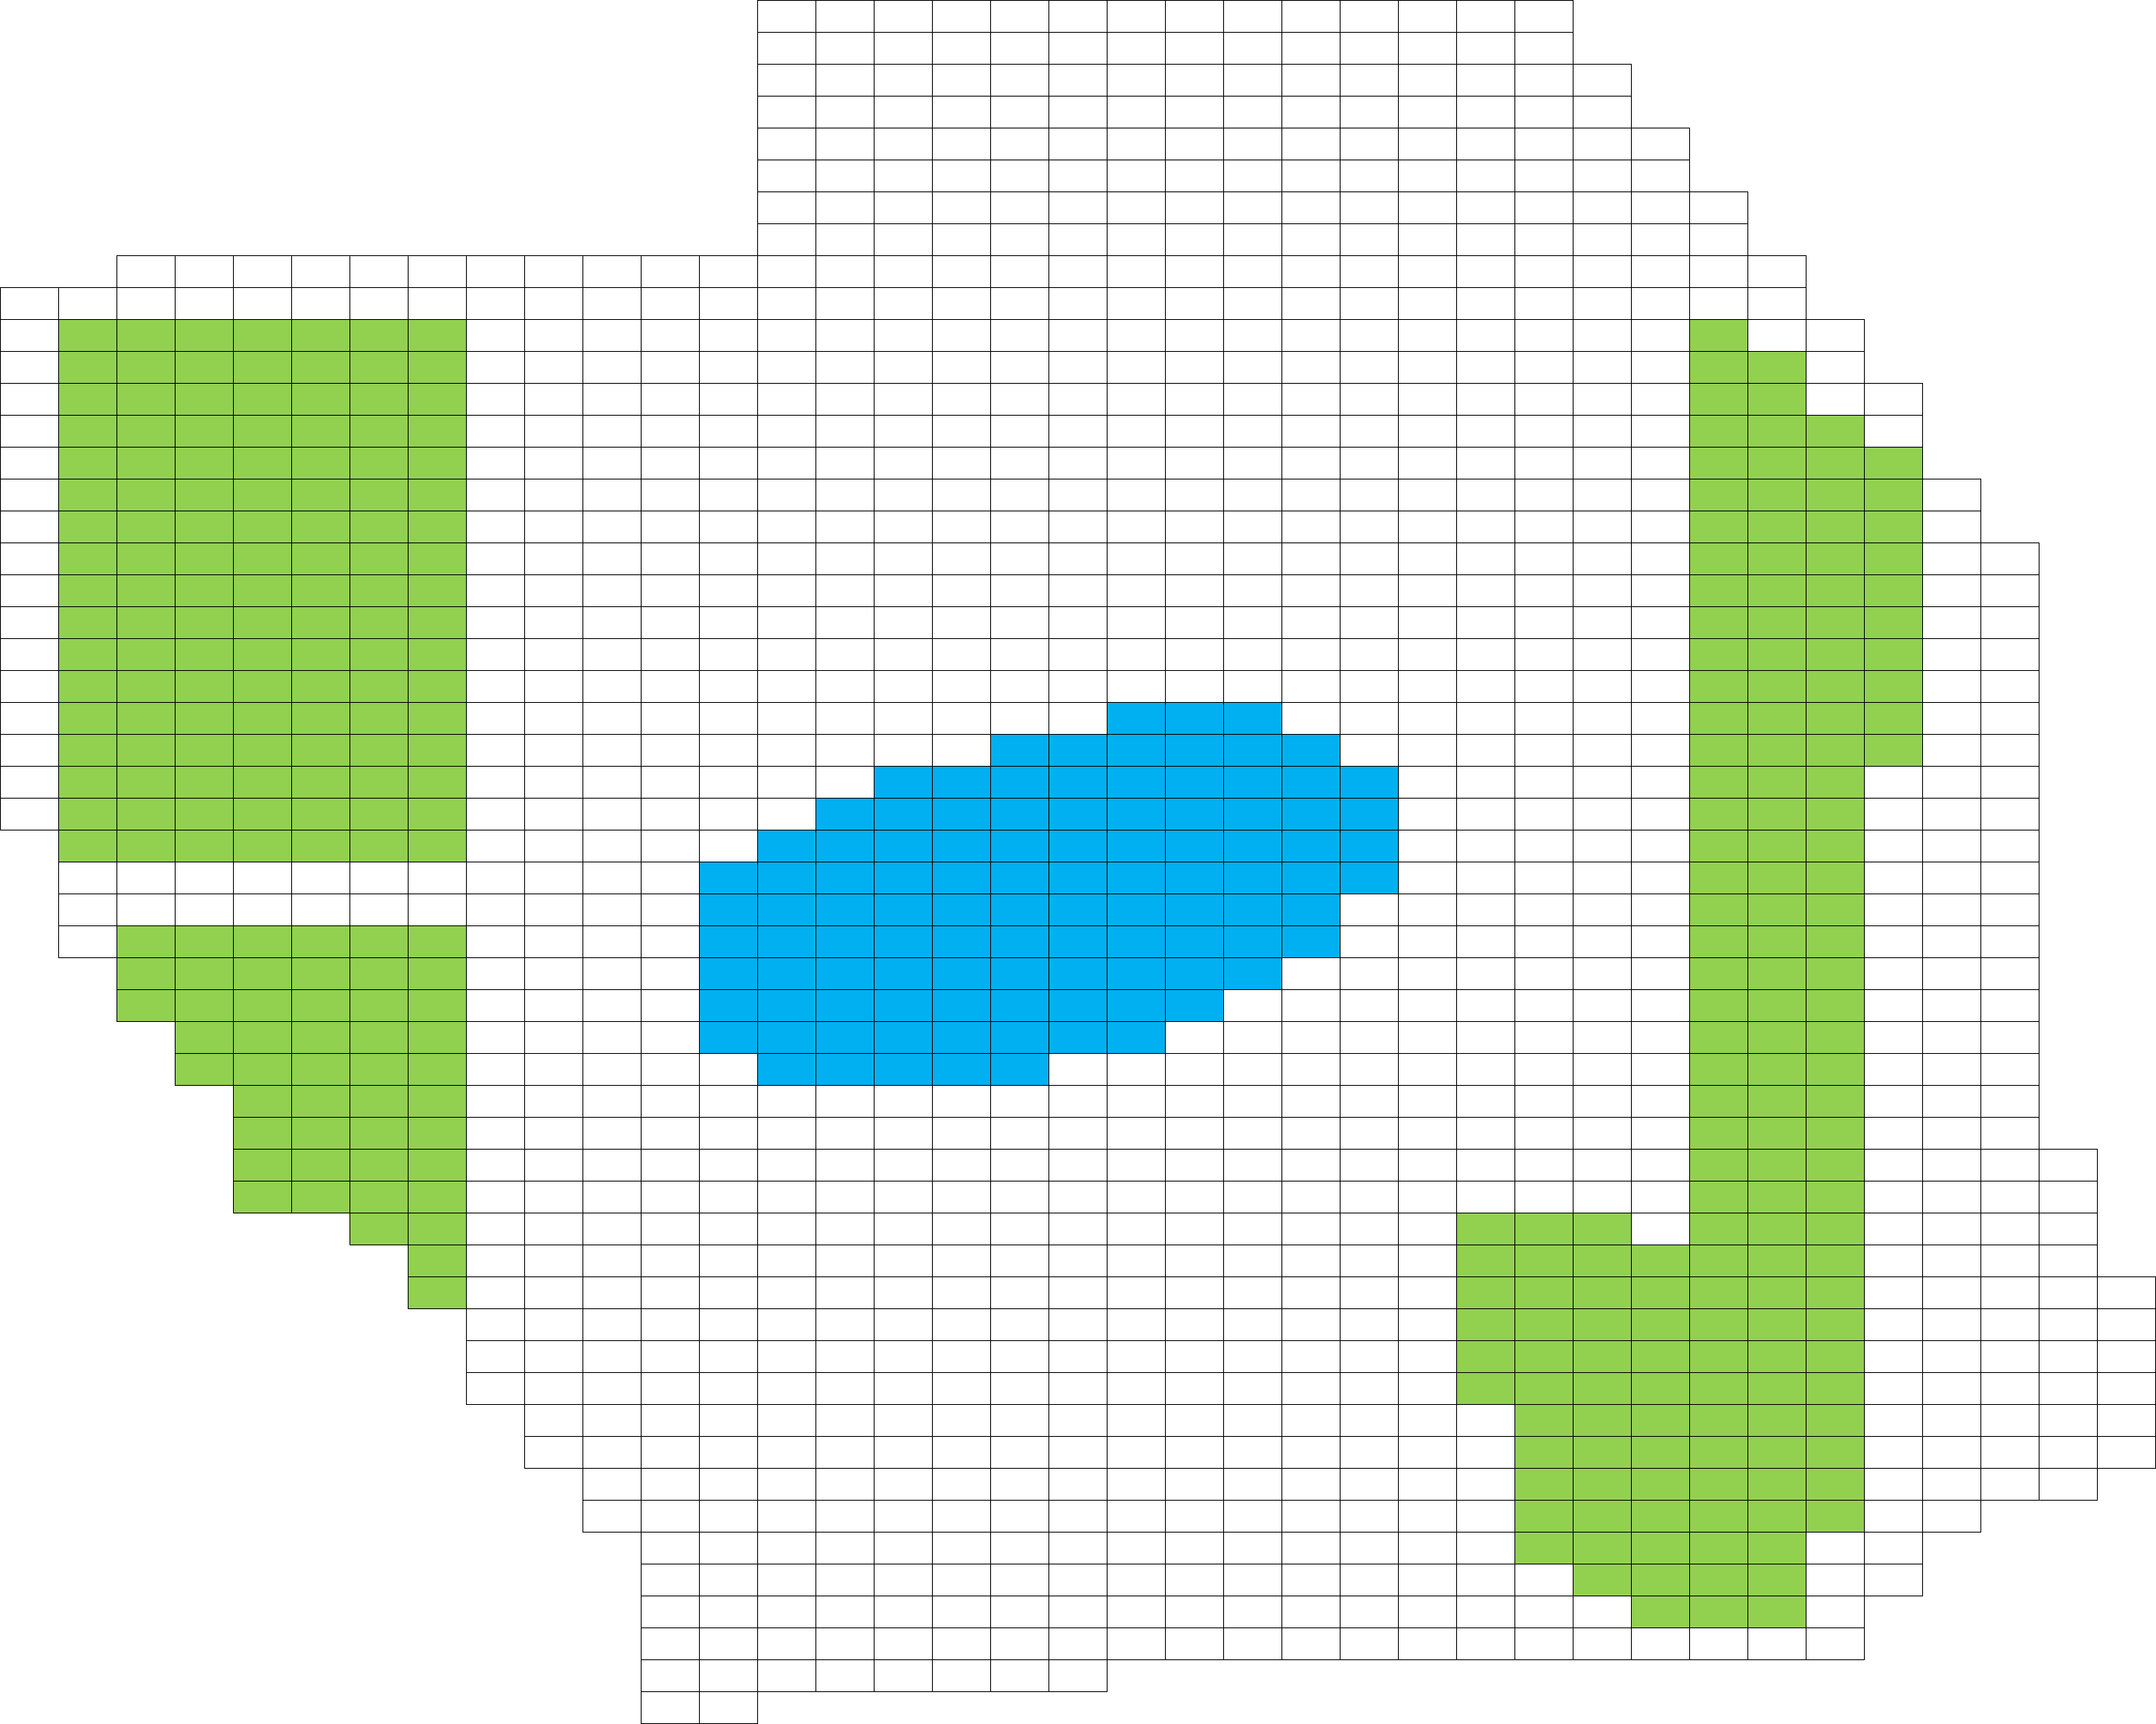
\includegraphics[width=\linewidth]{./figure/figureGood1}
            \caption{Reasonable Configuration}
            \label{fg1}
        \end{minipage}
        \begin{minipage}{0.3\linewidth}
            \centering
            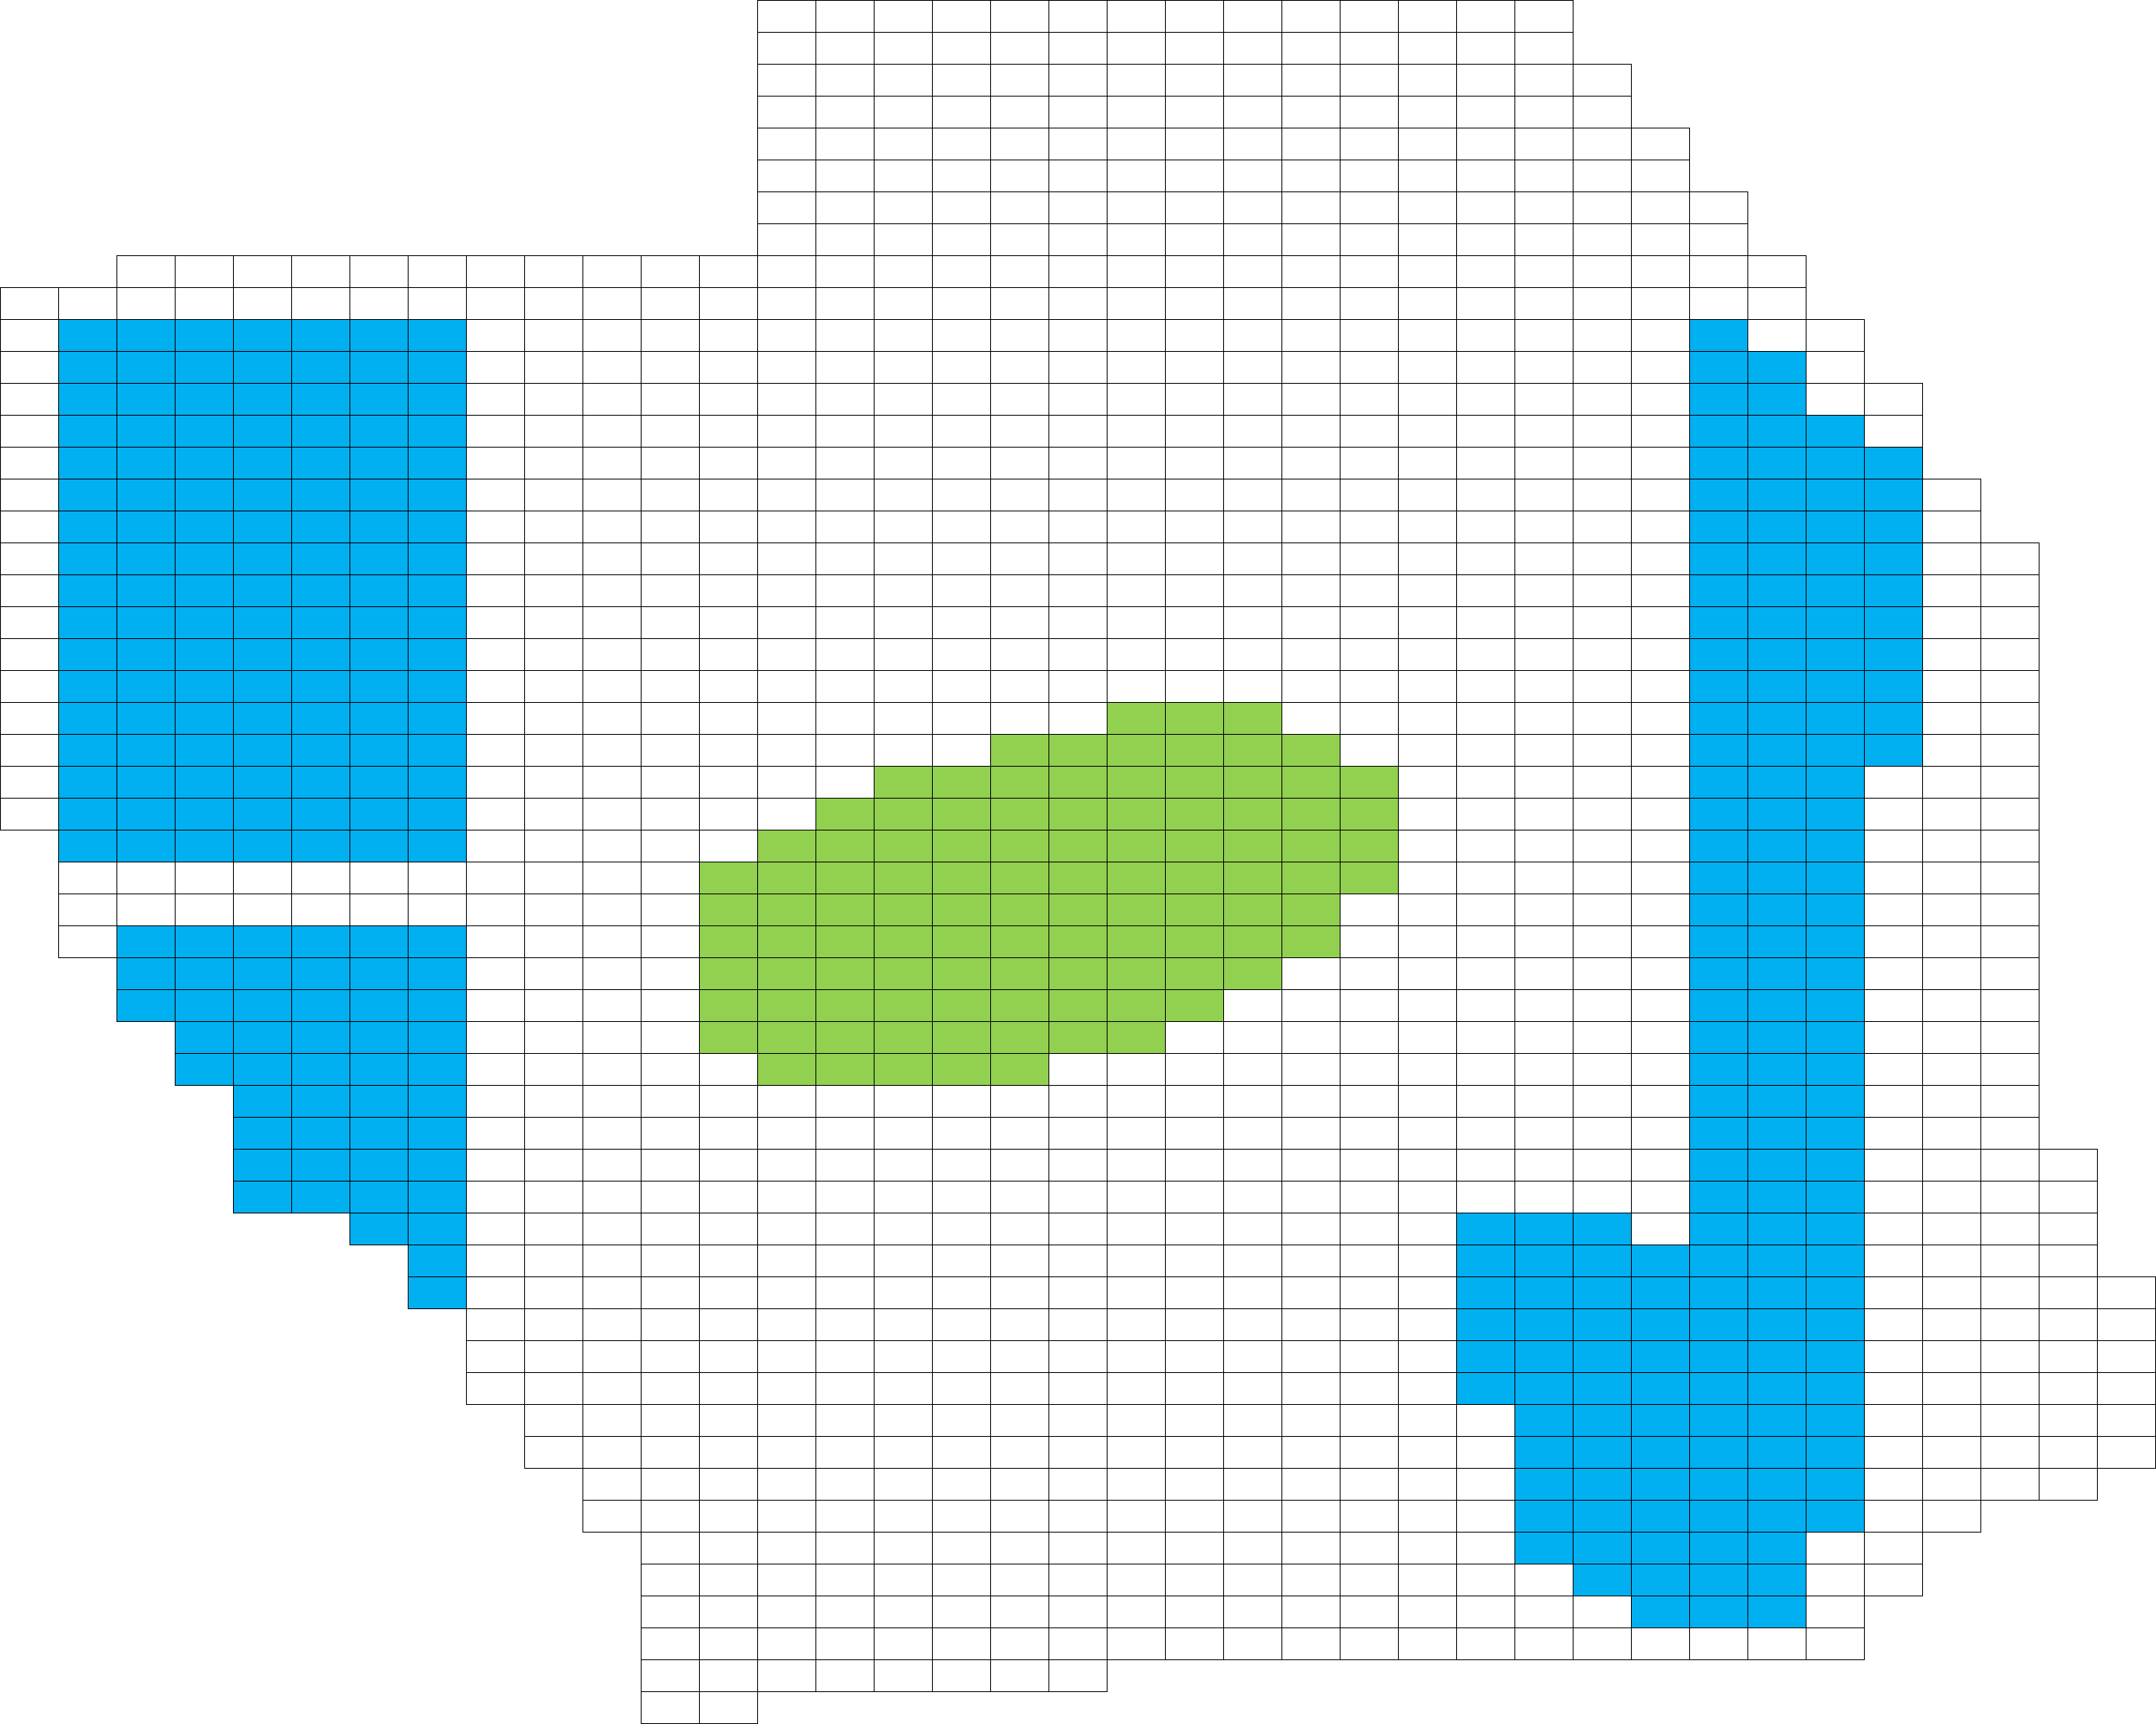
\includegraphics[width=\linewidth]{./figure/figureBad1}
            \caption{Swapped Configuration}
            \label{fb1}
        \end{minipage}
    \end{figure}

    The blue part is the cross-country skiing facility, and the green part is the crop farm.
    The two outputs of the algorithm are:

    Score of the reasonable solution: 28619($69.4$ pts)

    Score of the swapped solution: 19671($47.7$ pts)

    The second pair of facility is the regenerative farm and the agritourist center.
    We divide three parts of the land according to its slope as well.
    We first put the agritourist center to the single one with greater slope, while the regenerative farm were
    put to gentler lands, which is obviously better than the swapped ones.
    Then we swap them.
    The detailed configurations are as follows:

    \begin{figure}[H]
        \centering
        \begin{minipage}{0.3\linewidth}
            \centering
            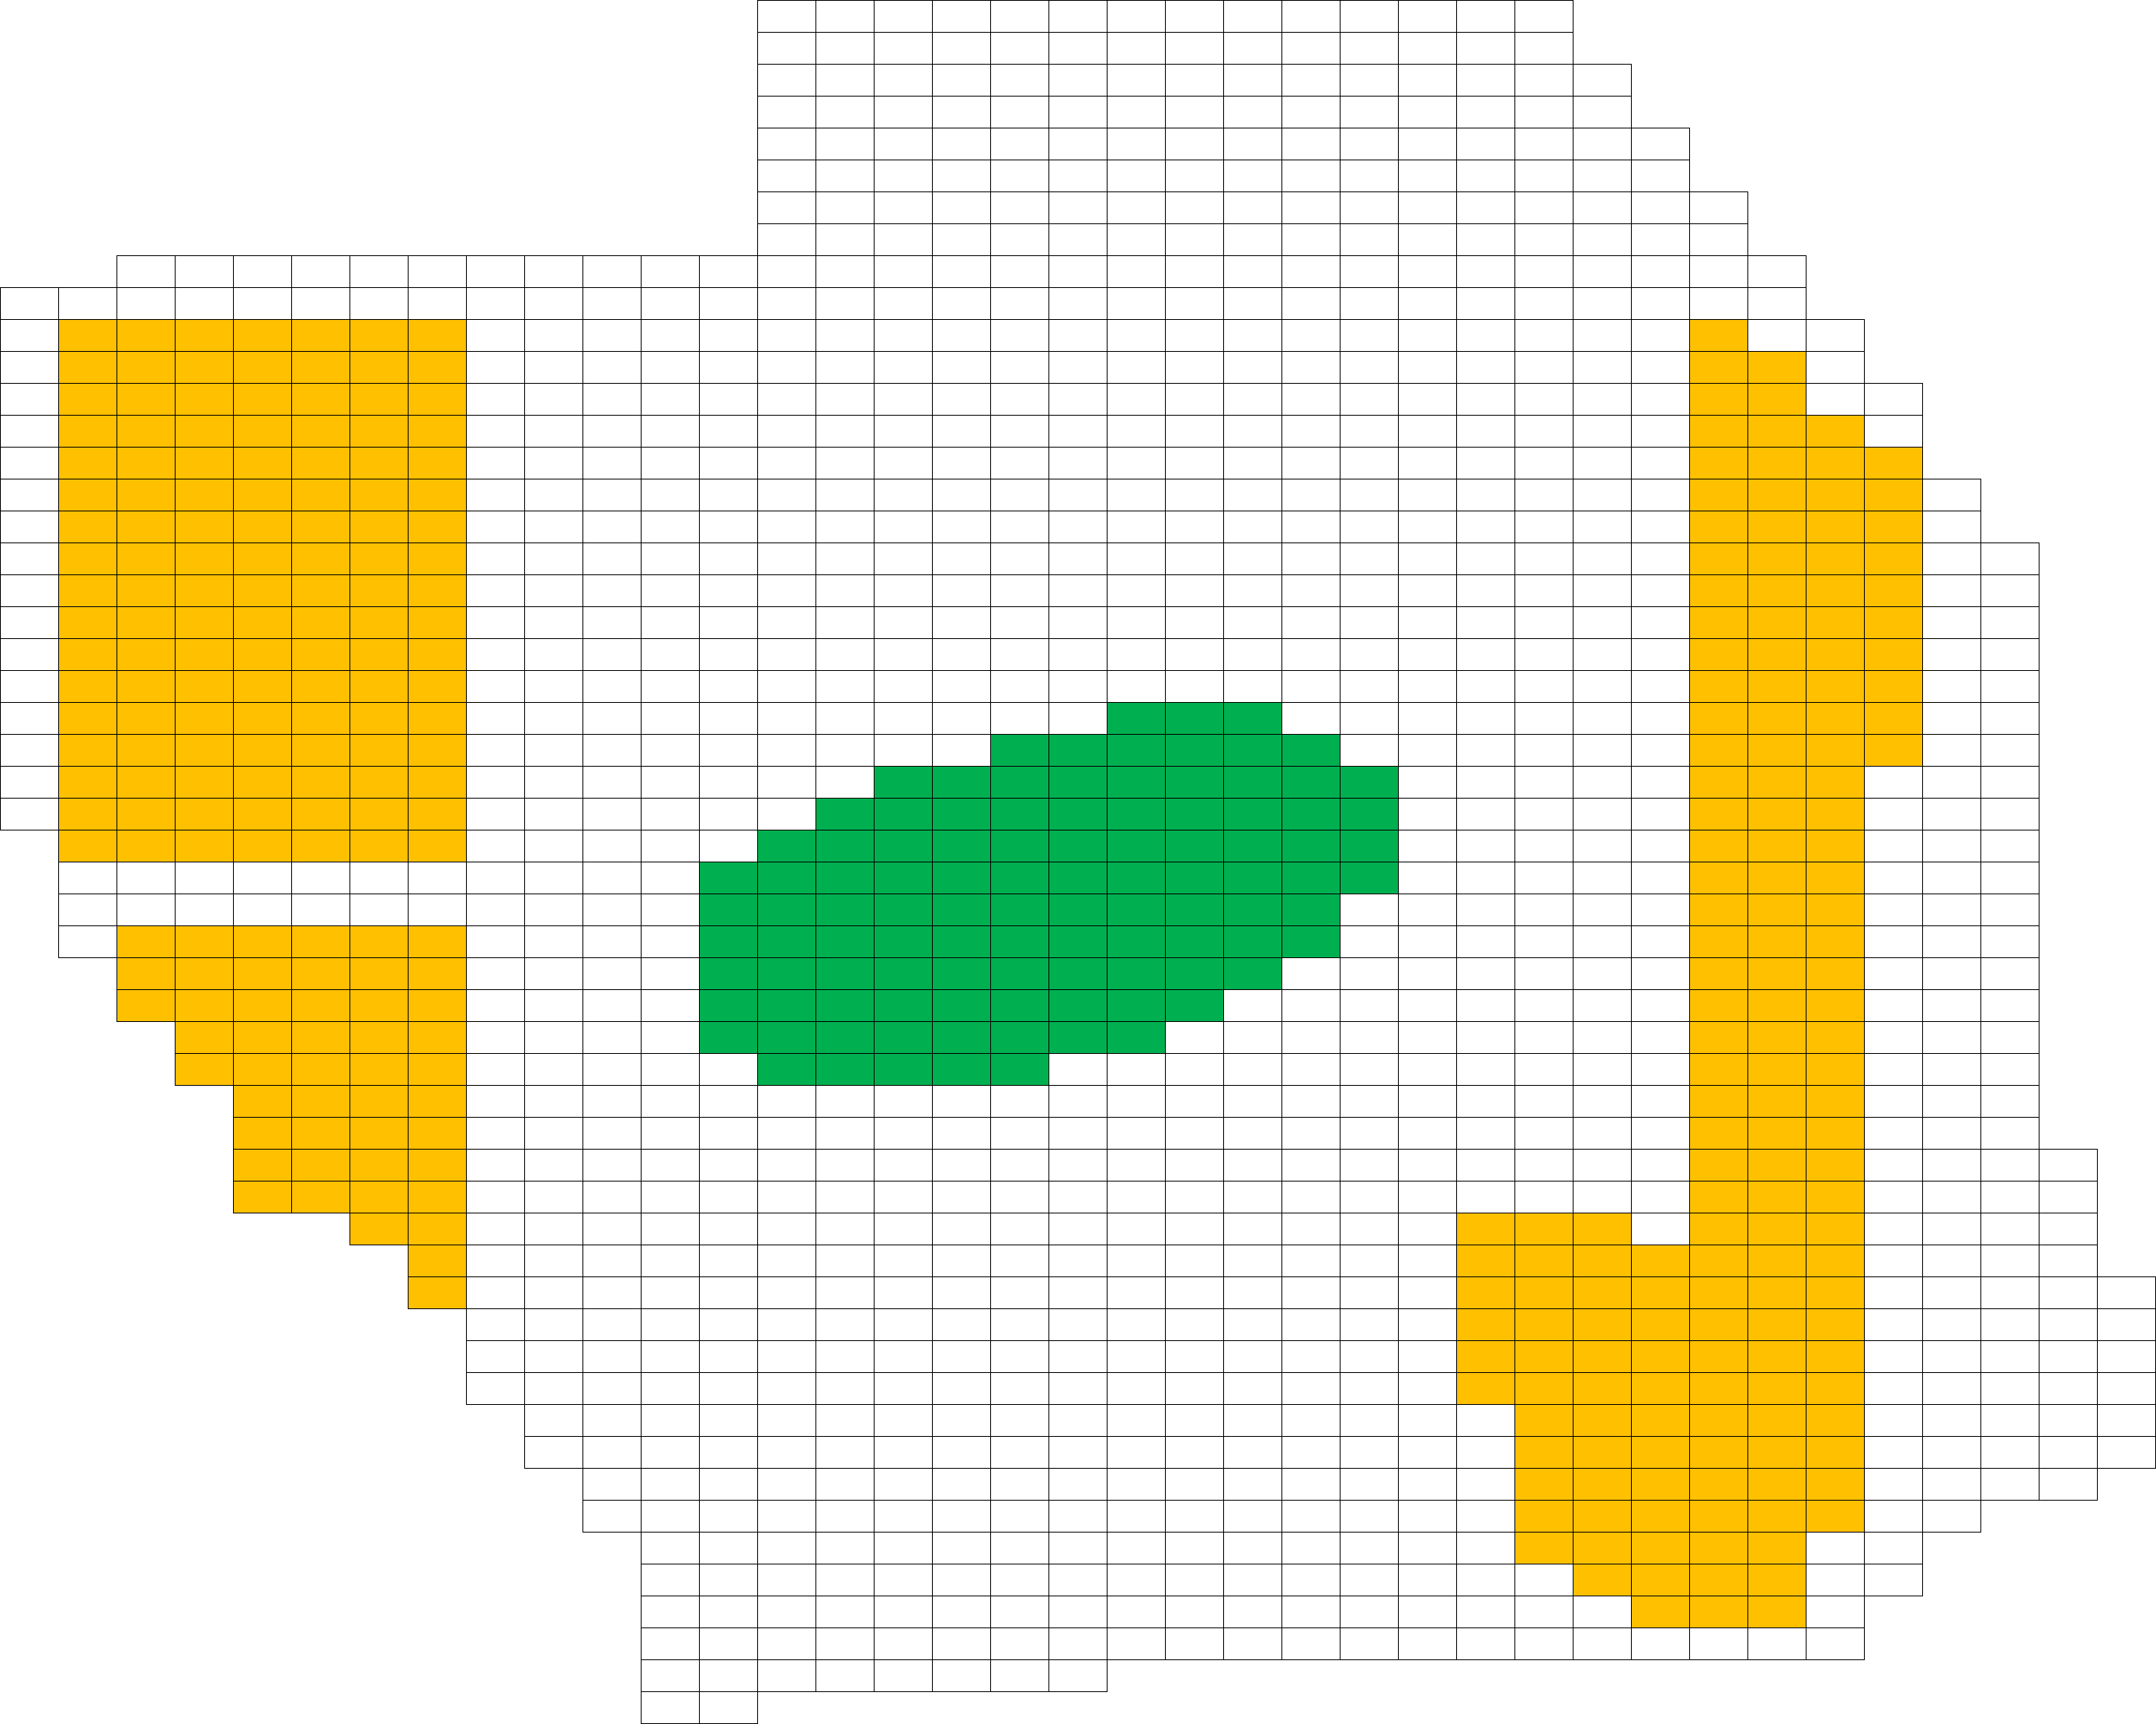
\includegraphics[width=\linewidth]{./figure/figureGood2}
            \caption{Reasonable Configuration}
            \label{fg2}
        \end{minipage}
        \begin{minipage}{0.3\linewidth}
            \centering
            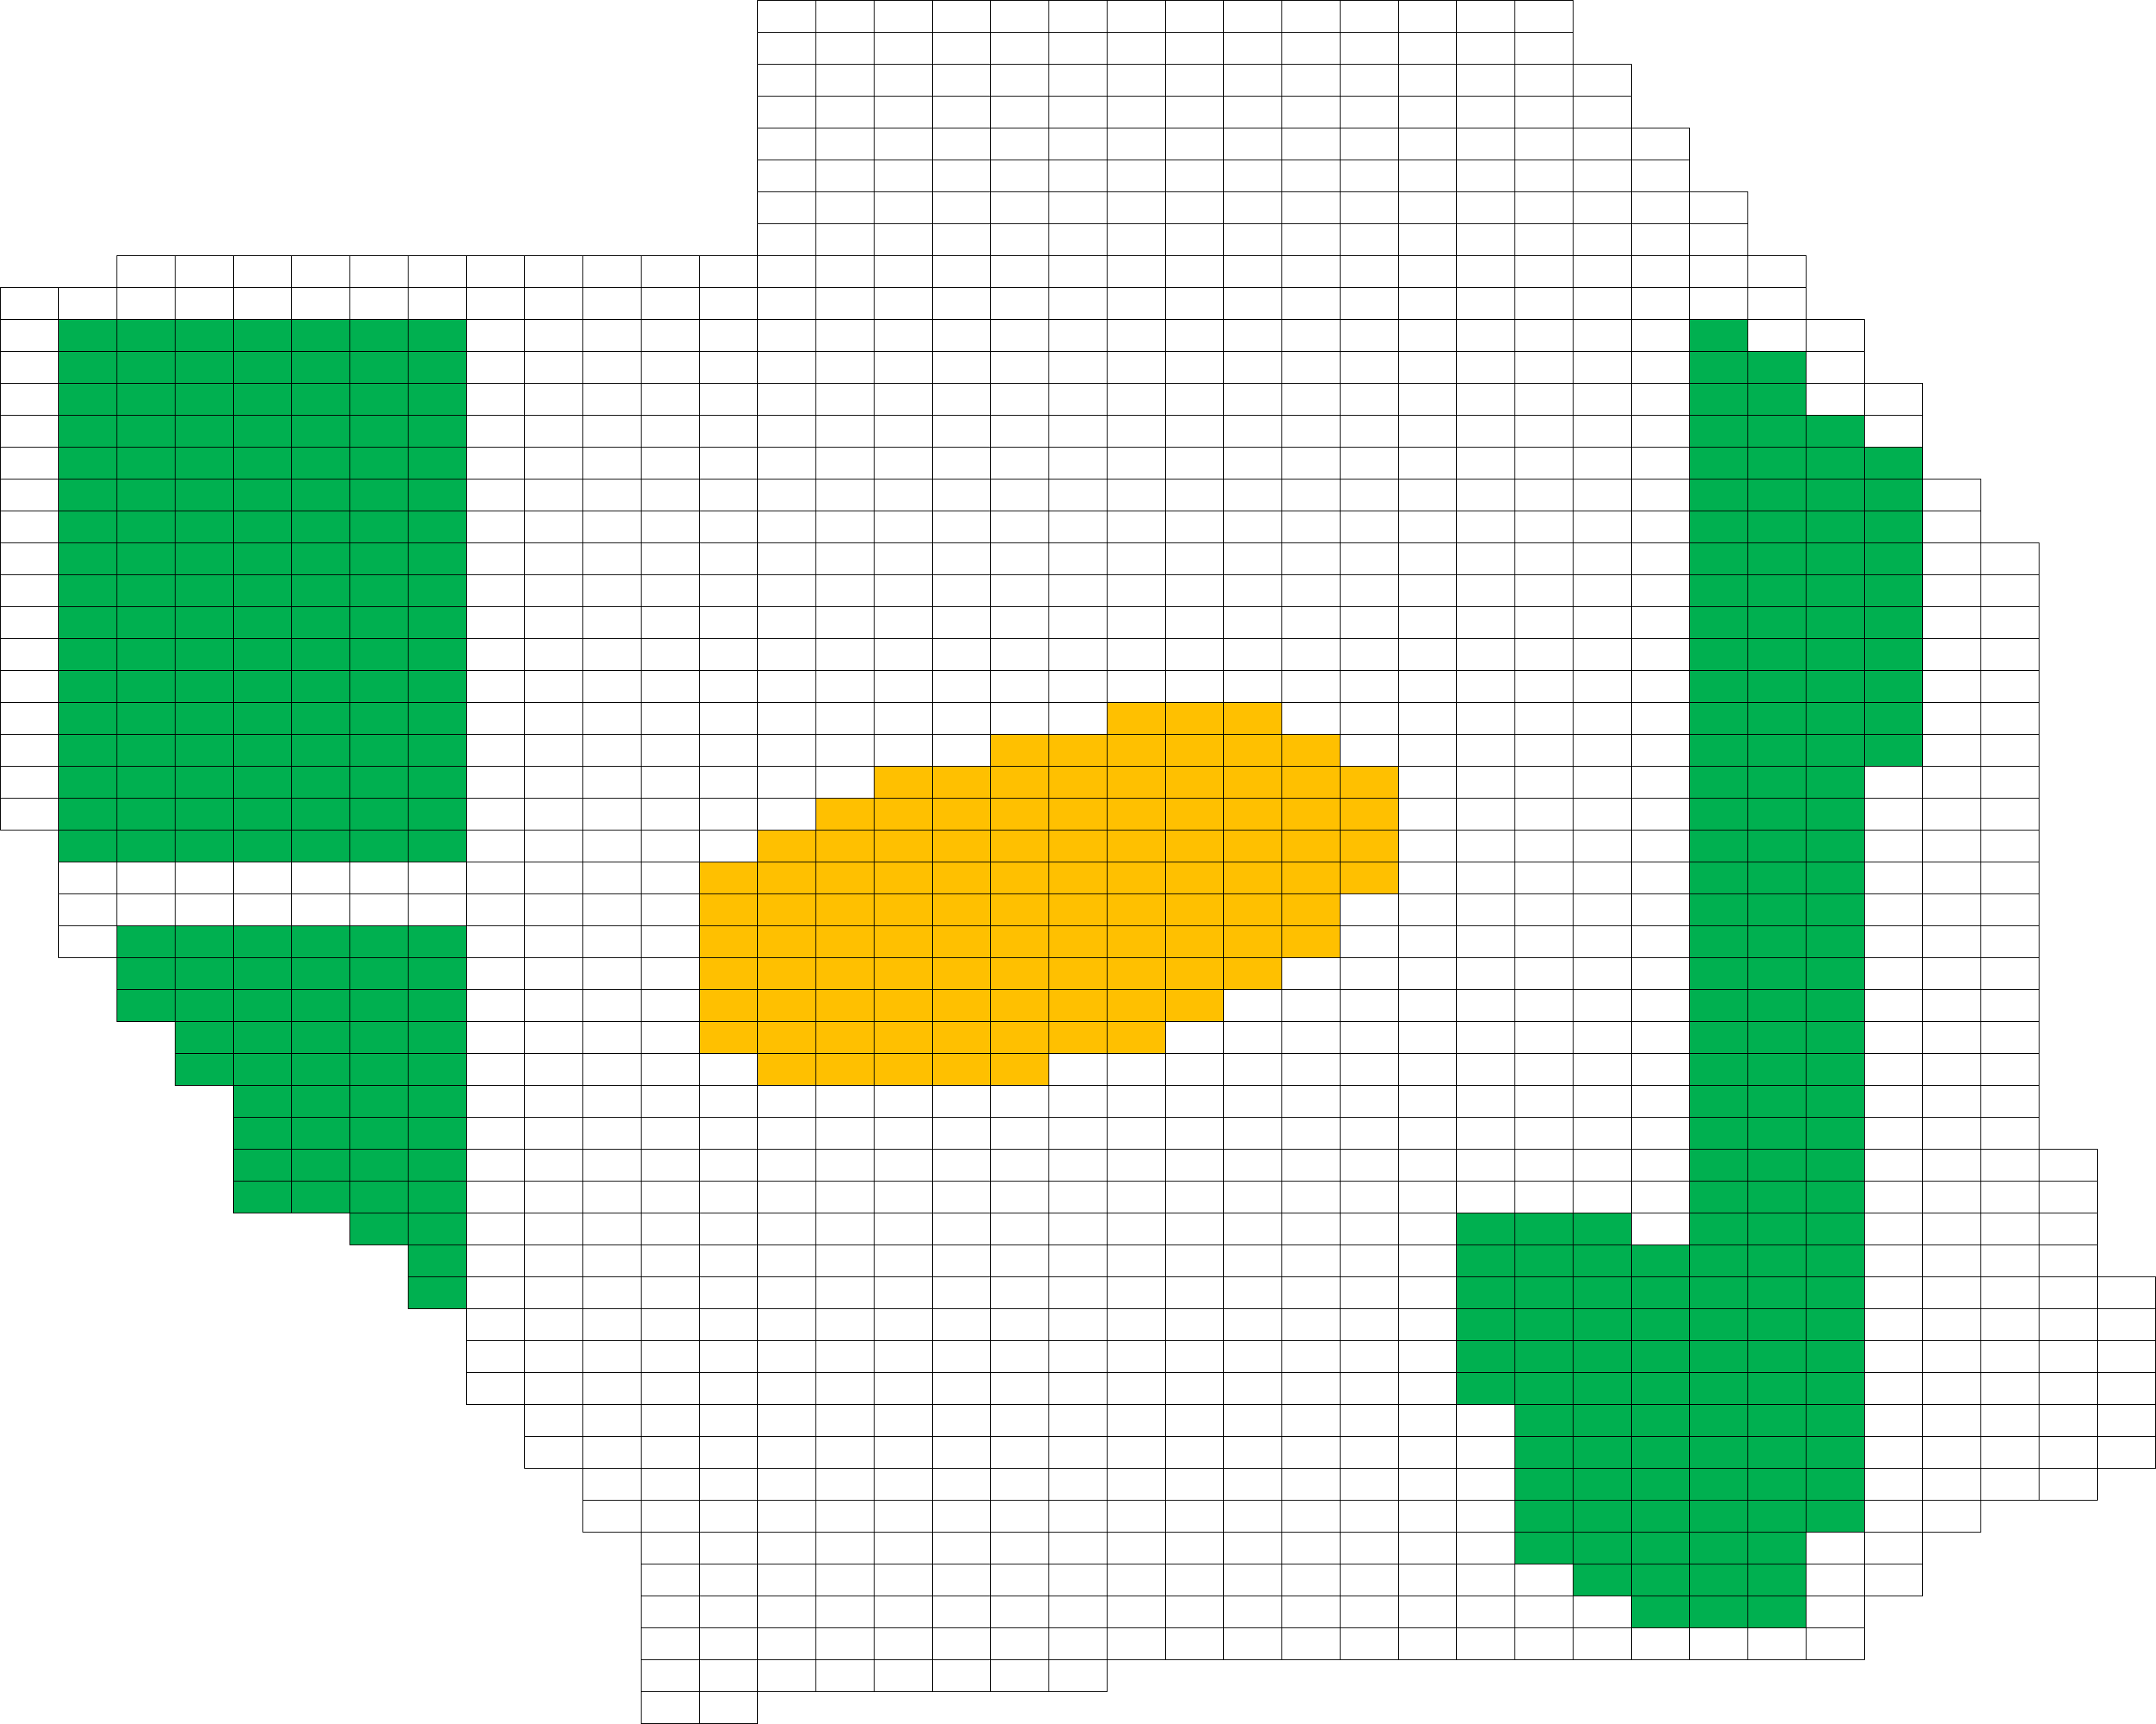
\includegraphics[width=\linewidth]{./figure/figureBad2}
            \caption{Swapped Configuration}
            \label{fb2}
        \end{minipage}
    \end{figure}

    The orange part is the regenerative farm, and the dark green part is the agritourist center.
    The two outputs of the algorithm are:

    Score of the reasonable solution: 26368($64.3$ pts)

    Score of the swapped solution: 18510($44.9$pts)

\end{document}